\section{Introdução}

\begin{frame}
  \begin{block}{Objetivos}
    \begin{itemize}
      \item Explorar o uso de Redes Neurais Baseadas em Física (PINNs) como uma alternativa aos métodos tradicionais de simulação de sistemas dinâmicos;
      \item embarcar uma PINN em um microcontrolador de baixo custo.
    \end{itemize}
  \end{block}

  \begin{block}{Relevância}
    \begin{itemize}
      \item Velocidade é essencial em aplicações que exigem alta velocidade e respostas em tempo real, como no Controle Preditivo Baseado em Modelo (MPC).
      \item Hardware de baixo custo torna a tecnologia viável para mais aplicações, inclusive em contextos industriais e acadêmicos.
    \end{itemize}
  \end{block}
\end{frame}

\begin{frame}{Problema Exemplo}
  \begin{columns}
    \begin{column}{0.4\textwidth}
      \begin{figure}
        \centering
        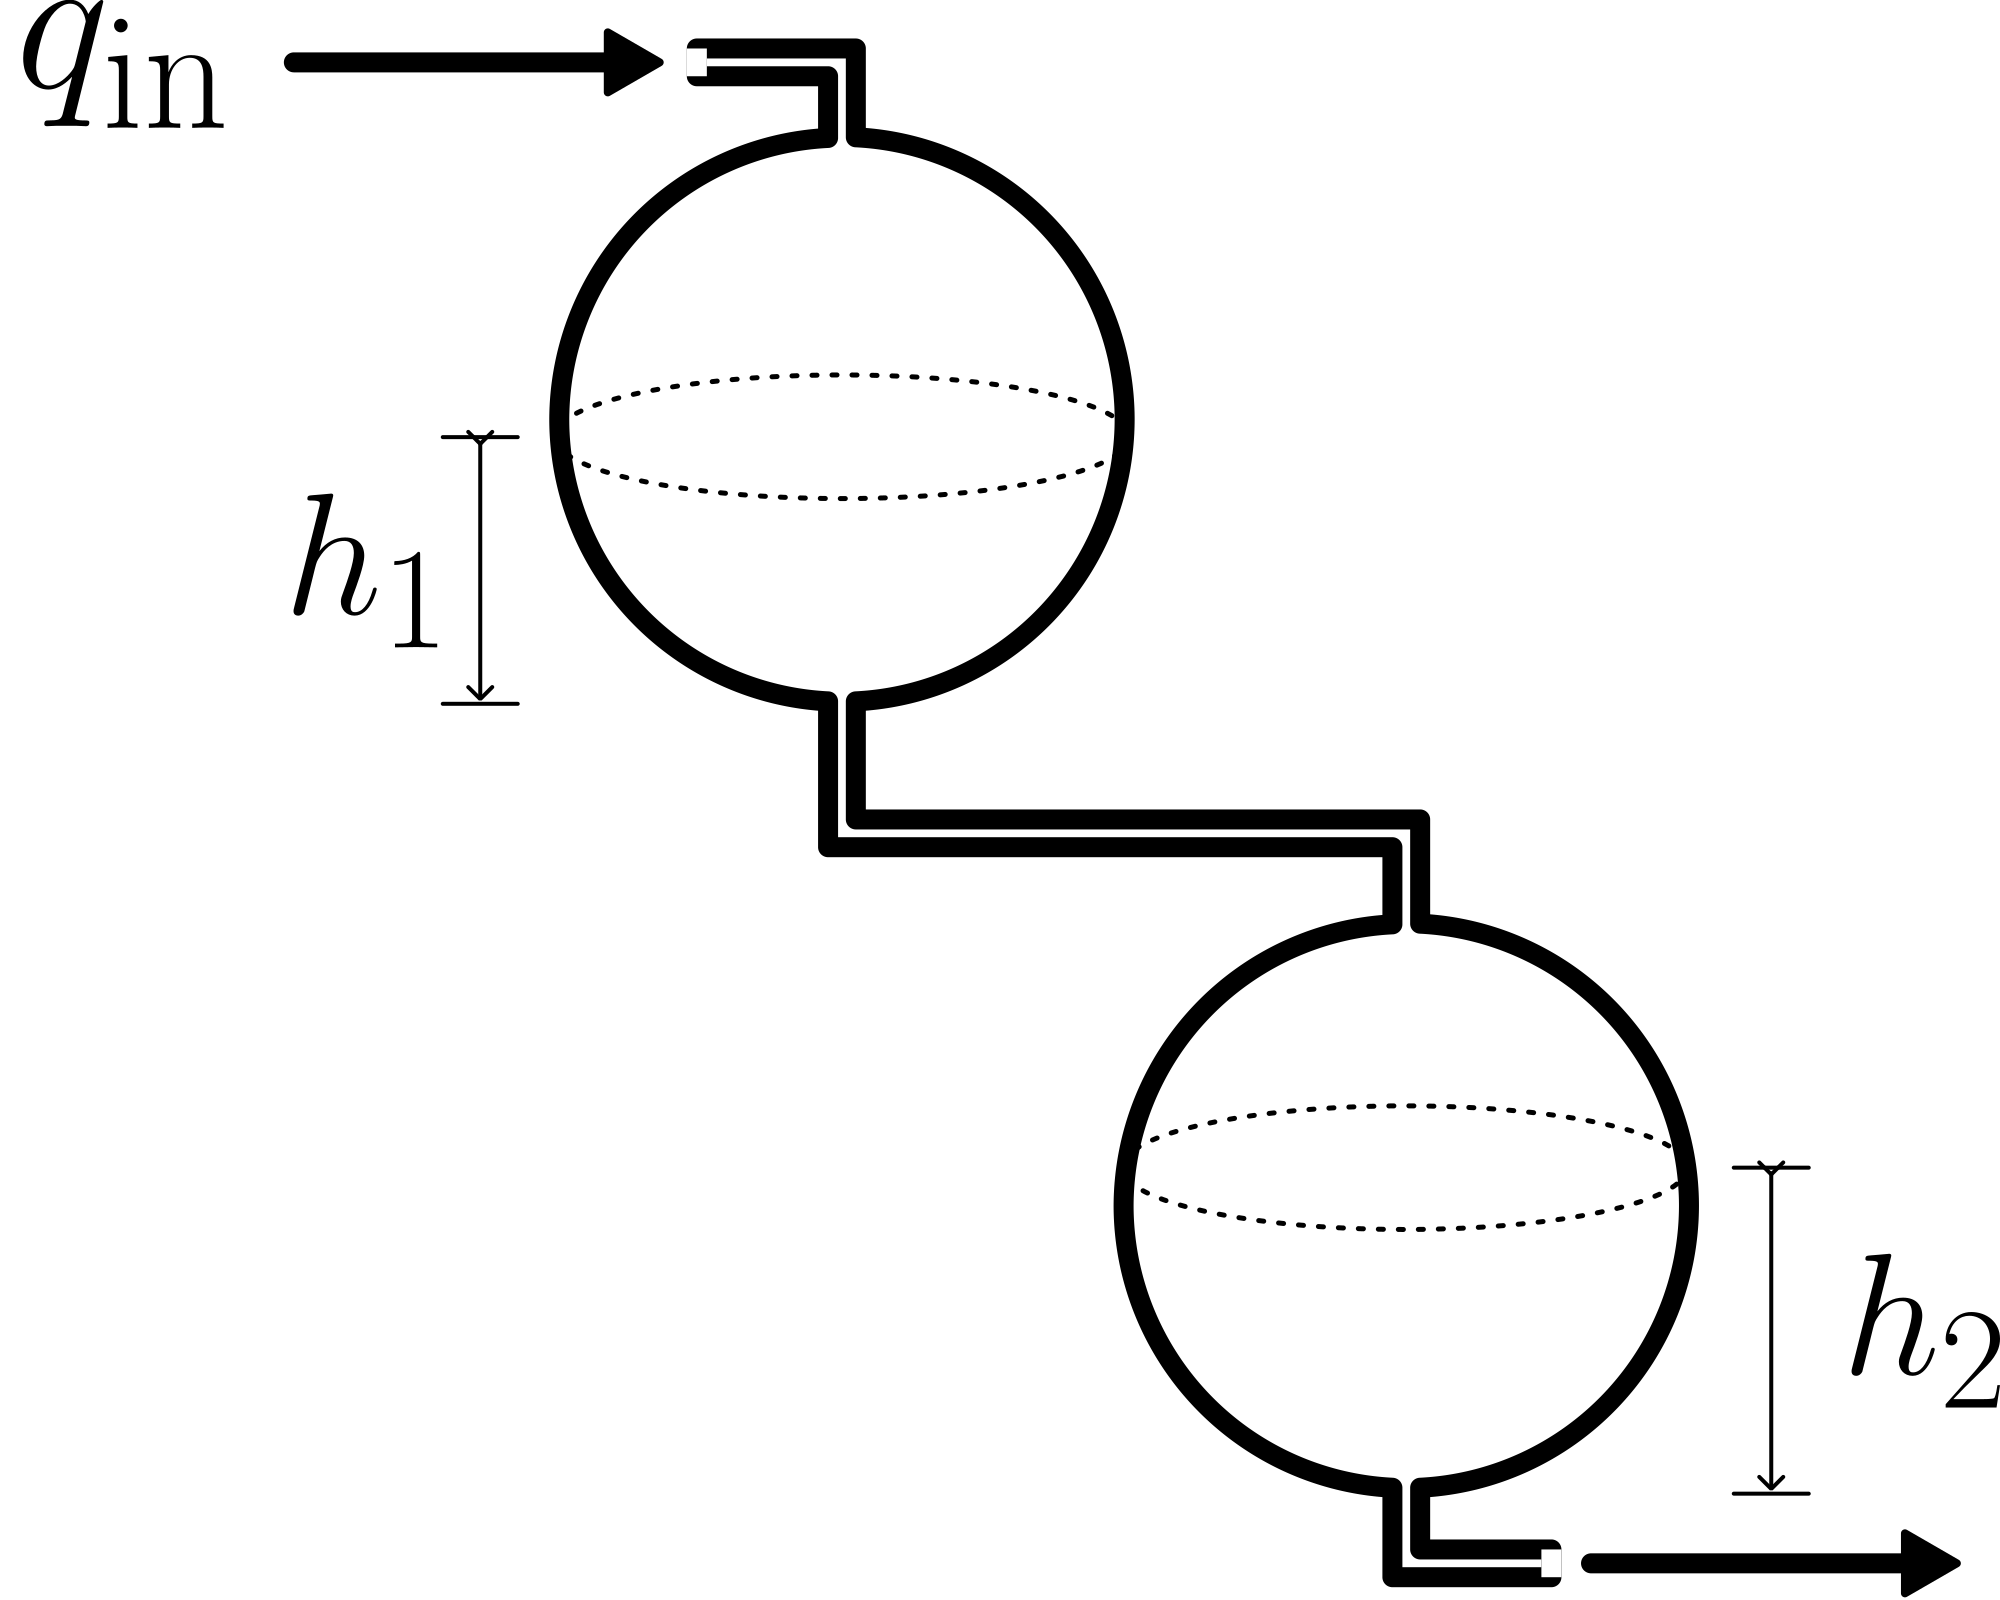
\includegraphics[width=\textwidth]{tank-system.png}
        \caption{Representação esquemática do sistema de dois tanques esféricos.}
        \label{fig:tank-system}
      \end{figure}
    \end{column}
    \begin{column}{0.6\textwidth}
      \begin{block}{Sistema de equações diferenciais dos tanques \parencite{wildson_2024}}
        \begin{subequations}
  \begin{align}
    \diff{h_1(t)}{t} & =
    \frac{
      q_{\mathrm{in}} - \alpha_1 s_1 \sqrt{2gh_1}
    }{
      \pi (2 R h_1 - h_1^2)
    }
    \label{eq:tank_system_a} \\[10pt]
    \diff{h_2(t)}{t} & =
    \frac{
      \alpha_1 s_1 \sqrt{2gh_1} - \alpha_2 s_2 \sqrt{2gh_2}
    }{
      \pi (2 R h_2 - h_2^2)
    }
    \label{eq:tank_system_b}
  \end{align}
\end{subequations}

        \vspace{0cm}
      \end{block}
    \end{column}
  \end{columns}
\end{frame}

\begin{frame}
  \begin{table}[ht]
  \centering
  \caption{Constantes do sistema de equações~\ref{eq:tank_system}.}
  \label{tab:tanks_params}
  \begin{tabular}{ccc}
    Símbolo    & Descrição                          & Valor               \\ \hline
    $\alpha_1$ & Fator de correção 1                & $0.56$              \\
    $\alpha_2$ & Fator de correção 2                & $0.30$              \\
    $s_1$      & Área da seção de saída do tanque 1 & $0.50 \, cm^2$      \\
    $s_2$      & Área da seção de saída do tanque 2 & $0.50 \, cm^2$      \\
    $g$        & Aceleração da gravidade            & $980.665 \, cm/s^2$ \\
    $R$        & Raio dos tanques                   & $14.85 \, cm$       \\ \hline
  \end{tabular}
\end{table}
\end{frame}

\begin{frame}{Mas, o que são PINNs?}
  \begin{columns}
    \begin{column}{0.5\textwidth}
      Introduzidas por \citeauthor{raissi_2017_I} em \citedate{raissi_2017_I}, as PINNs são uma forma de integrar princípios físicos ao treinamento de redes neurais. Elas têm o potencial de:
      \begin{itemize}
        \item Acelerar simulações em relação aos métodos numéricos tradicionais;
        \item melhorar a qualidade das previsões em comparação com redes neurais convencionais.
      \end{itemize}
    \end{column}
    \begin{column}{0.5\textwidth}
      \begin{figure}
        \centering
        \resizebox{\textwidth}{!}{% Graphic for TeX using PGF
% Title: /home/silas/Downloads/prh-35.1/slide-1/figures/neural-network.dia
% Creator: Dia v0.97+git
% CreationDate: Tue Aug  6 15:17:58 2024
% For: silas
% \usepackage{tikz}
% The following commands are not supported in PSTricks at present
% We define them conditionally, so when they are implemented,
% this pgf file will use them.
\ifx\du\undefined
  \newlength{\du}
\fi
\setlength{\du}{15\unitlength}
\begin{tikzpicture}[even odd rule]
  \pgftransformxscale{1.000000}
  \pgftransformyscale{-1.000000}
  \definecolor{dialinecolor}{rgb}{0.000000, 0.000000, 0.000000}
  \pgfsetstrokecolor{dialinecolor}
  \pgfsetstrokeopacity{1.000000}
  \definecolor{diafillcolor}{rgb}{1.000000, 1.000000, 1.000000}
  \pgfsetfillcolor{diafillcolor}
  \pgfsetfillopacity{1.000000}
  \pgfsetlinewidth{0.100000\du}
  \pgfsetdash{}{0pt}
  \pgfsetmiterjoin
  \definecolor{diafillcolor}{rgb}{1.000000, 1.000000, 1.000000}
  \pgfsetfillcolor{diafillcolor}
  \pgfsetfillopacity{1.000000}
  \pgfpathellipse{\pgfpoint{16.000000\du}{17.500000\du}}{\pgfpoint{1.000000\du}{0\du}}{\pgfpoint{0\du}{1.000000\du}}
  \pgfusepath{fill}
  \definecolor{dialinecolor}{rgb}{0.000000, 0.000000, 0.000000}
  \pgfsetstrokecolor{dialinecolor}
  \pgfsetstrokeopacity{1.000000}
  \pgfpathellipse{\pgfpoint{16.000000\du}{17.500000\du}}{\pgfpoint{1.000000\du}{0\du}}{\pgfpoint{0\du}{1.000000\du}}
  \pgfusepath{stroke}
  % setfont left to latex
  \definecolor{dialinecolor}{rgb}{0.000000, 0.000000, 0.000000}
  \pgfsetstrokecolor{dialinecolor}
  \pgfsetstrokeopacity{1.000000}
  \definecolor{diafillcolor}{rgb}{0.000000, 0.000000, 0.000000}
  \pgfsetfillcolor{diafillcolor}
  \pgfsetfillopacity{1.000000}
  \node[anchor=base,inner sep=0pt, outer sep=0pt,color=dialinecolor] at (16.000000\du,17.694063\du){$x_1$};
  \pgfsetlinewidth{0.100000\du}
  \pgfsetdash{}{0pt}
  \pgfsetmiterjoin
  \definecolor{diafillcolor}{rgb}{1.000000, 1.000000, 1.000000}
  \pgfsetfillcolor{diafillcolor}
  \pgfsetfillopacity{1.000000}
  \pgfpathellipse{\pgfpoint{16.000000\du}{20.500000\du}}{\pgfpoint{1.000000\du}{0\du}}{\pgfpoint{0\du}{1.000000\du}}
  \pgfusepath{fill}
  \definecolor{dialinecolor}{rgb}{0.000000, 0.000000, 0.000000}
  \pgfsetstrokecolor{dialinecolor}
  \pgfsetstrokeopacity{1.000000}
  \pgfpathellipse{\pgfpoint{16.000000\du}{20.500000\du}}{\pgfpoint{1.000000\du}{0\du}}{\pgfpoint{0\du}{1.000000\du}}
  \pgfusepath{stroke}
  % setfont left to latex
  \definecolor{dialinecolor}{rgb}{0.000000, 0.000000, 0.000000}
  \pgfsetstrokecolor{dialinecolor}
  \pgfsetstrokeopacity{1.000000}
  \definecolor{diafillcolor}{rgb}{0.000000, 0.000000, 0.000000}
  \pgfsetfillcolor{diafillcolor}
  \pgfsetfillopacity{1.000000}
  \node[anchor=base,inner sep=0pt, outer sep=0pt,color=dialinecolor] at (16.000000\du,20.694063\du){$x_2$};
  \pgfsetlinewidth{0.100000\du}
  \pgfsetdash{}{0pt}
  \pgfsetmiterjoin
  \definecolor{diafillcolor}{rgb}{1.000000, 1.000000, 1.000000}
  \pgfsetfillcolor{diafillcolor}
  \pgfsetfillopacity{1.000000}
  \pgfpathellipse{\pgfpoint{16.000000\du}{23.500000\du}}{\pgfpoint{1.000000\du}{0\du}}{\pgfpoint{0\du}{1.000000\du}}
  \pgfusepath{fill}
  \definecolor{dialinecolor}{rgb}{0.000000, 0.000000, 0.000000}
  \pgfsetstrokecolor{dialinecolor}
  \pgfsetstrokeopacity{1.000000}
  \pgfpathellipse{\pgfpoint{16.000000\du}{23.500000\du}}{\pgfpoint{1.000000\du}{0\du}}{\pgfpoint{0\du}{1.000000\du}}
  \pgfusepath{stroke}
  % setfont left to latex
  \definecolor{dialinecolor}{rgb}{0.000000, 0.000000, 0.000000}
  \pgfsetstrokecolor{dialinecolor}
  \pgfsetstrokeopacity{1.000000}
  \definecolor{diafillcolor}{rgb}{0.000000, 0.000000, 0.000000}
  \pgfsetfillcolor{diafillcolor}
  \pgfsetfillopacity{1.000000}
  \node[anchor=base,inner sep=0pt, outer sep=0pt,color=dialinecolor] at (16.000000\du,23.694063\du){$x_3$};
  \pgfsetlinewidth{0.100000\du}
  \pgfsetdash{}{0pt}
  \pgfsetmiterjoin
  \definecolor{diafillcolor}{rgb}{1.000000, 1.000000, 1.000000}
  \pgfsetfillcolor{diafillcolor}
  \pgfsetfillopacity{1.000000}
  \pgfpathellipse{\pgfpoint{21.000000\du}{16.000000\du}}{\pgfpoint{1.000000\du}{0\du}}{\pgfpoint{0\du}{1.000000\du}}
  \pgfusepath{fill}
  \definecolor{dialinecolor}{rgb}{0.000000, 0.000000, 0.000000}
  \pgfsetstrokecolor{dialinecolor}
  \pgfsetstrokeopacity{1.000000}
  \pgfpathellipse{\pgfpoint{21.000000\du}{16.000000\du}}{\pgfpoint{1.000000\du}{0\du}}{\pgfpoint{0\du}{1.000000\du}}
  \pgfusepath{stroke}
  % setfont left to latex
  \definecolor{dialinecolor}{rgb}{0.000000, 0.000000, 0.000000}
  \pgfsetstrokecolor{dialinecolor}
  \pgfsetstrokeopacity{1.000000}
  \definecolor{diafillcolor}{rgb}{0.000000, 0.000000, 0.000000}
  \pgfsetfillcolor{diafillcolor}
  \pgfsetfillopacity{1.000000}
  \node[anchor=base,inner sep=0pt, outer sep=0pt,color=dialinecolor] at (21.000000\du,16.194063\du){$\sum f$};
  \pgfsetlinewidth{0.100000\du}
  \pgfsetdash{}{0pt}
  \pgfsetbuttcap
  {
    \definecolor{diafillcolor}{rgb}{0.000000, 0.000000, 0.000000}
    \pgfsetfillcolor{diafillcolor}
    \pgfsetfillopacity{1.000000}
    % was here!!!
    \pgfsetarrowsend{stealth}
    \definecolor{dialinecolor}{rgb}{0.000000, 0.000000, 0.000000}
    \pgfsetstrokecolor{dialinecolor}
    \pgfsetstrokeopacity{1.000000}
    \draw (17.000000\du,17.500000\du)--(20.000000\du,16.000000\du);
  }
  \pgfsetlinewidth{0.100000\du}
  \pgfsetdash{}{0pt}
  \pgfsetmiterjoin
  \definecolor{diafillcolor}{rgb}{1.000000, 1.000000, 1.000000}
  \pgfsetfillcolor{diafillcolor}
  \pgfsetfillopacity{1.000000}
  \pgfpathellipse{\pgfpoint{21.000000\du}{19.000000\du}}{\pgfpoint{1.000000\du}{0\du}}{\pgfpoint{0\du}{1.000000\du}}
  \pgfusepath{fill}
  \definecolor{dialinecolor}{rgb}{0.000000, 0.000000, 0.000000}
  \pgfsetstrokecolor{dialinecolor}
  \pgfsetstrokeopacity{1.000000}
  \pgfpathellipse{\pgfpoint{21.000000\du}{19.000000\du}}{\pgfpoint{1.000000\du}{0\du}}{\pgfpoint{0\du}{1.000000\du}}
  \pgfusepath{stroke}
  % setfont left to latex
  \definecolor{dialinecolor}{rgb}{0.000000, 0.000000, 0.000000}
  \pgfsetstrokecolor{dialinecolor}
  \pgfsetstrokeopacity{1.000000}
  \definecolor{diafillcolor}{rgb}{0.000000, 0.000000, 0.000000}
  \pgfsetfillcolor{diafillcolor}
  \pgfsetfillopacity{1.000000}
  \node[anchor=base,inner sep=0pt, outer sep=0pt,color=dialinecolor] at (21.000000\du,19.194063\du){$\sum f$};
  \pgfsetlinewidth{0.100000\du}
  \pgfsetdash{}{0pt}
  \pgfsetmiterjoin
  \definecolor{diafillcolor}{rgb}{1.000000, 1.000000, 1.000000}
  \pgfsetfillcolor{diafillcolor}
  \pgfsetfillopacity{1.000000}
  \pgfpathellipse{\pgfpoint{21.000000\du}{22.000000\du}}{\pgfpoint{1.000000\du}{0\du}}{\pgfpoint{0\du}{1.000000\du}}
  \pgfusepath{fill}
  \definecolor{dialinecolor}{rgb}{0.000000, 0.000000, 0.000000}
  \pgfsetstrokecolor{dialinecolor}
  \pgfsetstrokeopacity{1.000000}
  \pgfpathellipse{\pgfpoint{21.000000\du}{22.000000\du}}{\pgfpoint{1.000000\du}{0\du}}{\pgfpoint{0\du}{1.000000\du}}
  \pgfusepath{stroke}
  % setfont left to latex
  \definecolor{dialinecolor}{rgb}{0.000000, 0.000000, 0.000000}
  \pgfsetstrokecolor{dialinecolor}
  \pgfsetstrokeopacity{1.000000}
  \definecolor{diafillcolor}{rgb}{0.000000, 0.000000, 0.000000}
  \pgfsetfillcolor{diafillcolor}
  \pgfsetfillopacity{1.000000}
  \node[anchor=base,inner sep=0pt, outer sep=0pt,color=dialinecolor] at (21.000000\du,22.194063\du){$\sum f$};
  \pgfsetlinewidth{0.100000\du}
  \pgfsetdash{}{0pt}
  \pgfsetmiterjoin
  \definecolor{diafillcolor}{rgb}{1.000000, 1.000000, 1.000000}
  \pgfsetfillcolor{diafillcolor}
  \pgfsetfillopacity{1.000000}
  \pgfpathellipse{\pgfpoint{21.000000\du}{25.000000\du}}{\pgfpoint{1.000000\du}{0\du}}{\pgfpoint{0\du}{1.000000\du}}
  \pgfusepath{fill}
  \definecolor{dialinecolor}{rgb}{0.000000, 0.000000, 0.000000}
  \pgfsetstrokecolor{dialinecolor}
  \pgfsetstrokeopacity{1.000000}
  \pgfpathellipse{\pgfpoint{21.000000\du}{25.000000\du}}{\pgfpoint{1.000000\du}{0\du}}{\pgfpoint{0\du}{1.000000\du}}
  \pgfusepath{stroke}
  % setfont left to latex
  \definecolor{dialinecolor}{rgb}{0.000000, 0.000000, 0.000000}
  \pgfsetstrokecolor{dialinecolor}
  \pgfsetstrokeopacity{1.000000}
  \definecolor{diafillcolor}{rgb}{0.000000, 0.000000, 0.000000}
  \pgfsetfillcolor{diafillcolor}
  \pgfsetfillopacity{1.000000}
  \node[anchor=base,inner sep=0pt, outer sep=0pt,color=dialinecolor] at (21.000000\du,25.194063\du){$\sum f$};
  \pgfsetlinewidth{0.100000\du}
  \pgfsetdash{}{0pt}
  \pgfsetmiterjoin
  \definecolor{diafillcolor}{rgb}{1.000000, 1.000000, 1.000000}
  \pgfsetfillcolor{diafillcolor}
  \pgfsetfillopacity{1.000000}
  \pgfpathellipse{\pgfpoint{26.000000\du}{17.500000\du}}{\pgfpoint{1.000000\du}{0\du}}{\pgfpoint{0\du}{1.000000\du}}
  \pgfusepath{fill}
  \definecolor{dialinecolor}{rgb}{0.000000, 0.000000, 0.000000}
  \pgfsetstrokecolor{dialinecolor}
  \pgfsetstrokeopacity{1.000000}
  \pgfpathellipse{\pgfpoint{26.000000\du}{17.500000\du}}{\pgfpoint{1.000000\du}{0\du}}{\pgfpoint{0\du}{1.000000\du}}
  \pgfusepath{stroke}
  % setfont left to latex
  \definecolor{dialinecolor}{rgb}{0.000000, 0.000000, 0.000000}
  \pgfsetstrokecolor{dialinecolor}
  \pgfsetstrokeopacity{1.000000}
  \definecolor{diafillcolor}{rgb}{0.000000, 0.000000, 0.000000}
  \pgfsetfillcolor{diafillcolor}
  \pgfsetfillopacity{1.000000}
  \node[anchor=base,inner sep=0pt, outer sep=0pt,color=dialinecolor] at (26.000000\du,17.694063\du){$\sum f$};
  \pgfsetlinewidth{0.100000\du}
  \pgfsetdash{}{0pt}
  \pgfsetmiterjoin
  \definecolor{diafillcolor}{rgb}{1.000000, 1.000000, 1.000000}
  \pgfsetfillcolor{diafillcolor}
  \pgfsetfillopacity{1.000000}
  \pgfpathellipse{\pgfpoint{26.000000\du}{20.500000\du}}{\pgfpoint{1.000000\du}{0\du}}{\pgfpoint{0\du}{1.000000\du}}
  \pgfusepath{fill}
  \definecolor{dialinecolor}{rgb}{0.000000, 0.000000, 0.000000}
  \pgfsetstrokecolor{dialinecolor}
  \pgfsetstrokeopacity{1.000000}
  \pgfpathellipse{\pgfpoint{26.000000\du}{20.500000\du}}{\pgfpoint{1.000000\du}{0\du}}{\pgfpoint{0\du}{1.000000\du}}
  \pgfusepath{stroke}
  % setfont left to latex
  \definecolor{dialinecolor}{rgb}{0.000000, 0.000000, 0.000000}
  \pgfsetstrokecolor{dialinecolor}
  \pgfsetstrokeopacity{1.000000}
  \definecolor{diafillcolor}{rgb}{0.000000, 0.000000, 0.000000}
  \pgfsetfillcolor{diafillcolor}
  \pgfsetfillopacity{1.000000}
  \node[anchor=base,inner sep=0pt, outer sep=0pt,color=dialinecolor] at (26.000000\du,20.694063\du){$\sum f$};
  \pgfsetlinewidth{0.100000\du}
  \pgfsetdash{}{0pt}
  \pgfsetmiterjoin
  \definecolor{diafillcolor}{rgb}{1.000000, 1.000000, 1.000000}
  \pgfsetfillcolor{diafillcolor}
  \pgfsetfillopacity{1.000000}
  \pgfpathellipse{\pgfpoint{26.000000\du}{23.500000\du}}{\pgfpoint{1.000000\du}{0\du}}{\pgfpoint{0\du}{1.000000\du}}
  \pgfusepath{fill}
  \definecolor{dialinecolor}{rgb}{0.000000, 0.000000, 0.000000}
  \pgfsetstrokecolor{dialinecolor}
  \pgfsetstrokeopacity{1.000000}
  \pgfpathellipse{\pgfpoint{26.000000\du}{23.500000\du}}{\pgfpoint{1.000000\du}{0\du}}{\pgfpoint{0\du}{1.000000\du}}
  \pgfusepath{stroke}
  % setfont left to latex
  \definecolor{dialinecolor}{rgb}{0.000000, 0.000000, 0.000000}
  \pgfsetstrokecolor{dialinecolor}
  \pgfsetstrokeopacity{1.000000}
  \definecolor{diafillcolor}{rgb}{0.000000, 0.000000, 0.000000}
  \pgfsetfillcolor{diafillcolor}
  \pgfsetfillopacity{1.000000}
  \node[anchor=base,inner sep=0pt, outer sep=0pt,color=dialinecolor] at (26.000000\du,23.694063\du){$\sum f$};
  \pgfsetlinewidth{0.100000\du}
  \pgfsetdash{}{0pt}
  \pgfsetmiterjoin
  \definecolor{diafillcolor}{rgb}{1.000000, 1.000000, 1.000000}
  \pgfsetfillcolor{diafillcolor}
  \pgfsetfillopacity{1.000000}
  \pgfpathellipse{\pgfpoint{31.000000\du}{16.000000\du}}{\pgfpoint{1.031260\du}{0\du}}{\pgfpoint{0\du}{1.031260\du}}
  \pgfusepath{fill}
  \definecolor{dialinecolor}{rgb}{0.000000, 0.000000, 0.000000}
  \pgfsetstrokecolor{dialinecolor}
  \pgfsetstrokeopacity{1.000000}
  \pgfpathellipse{\pgfpoint{31.000000\du}{16.000000\du}}{\pgfpoint{1.031260\du}{0\du}}{\pgfpoint{0\du}{1.031260\du}}
  \pgfusepath{stroke}
  % setfont left to latex
  \definecolor{dialinecolor}{rgb}{0.000000, 0.000000, 0.000000}
  \pgfsetstrokecolor{dialinecolor}
  \pgfsetstrokeopacity{1.000000}
  \definecolor{diafillcolor}{rgb}{0.000000, 0.000000, 0.000000}
  \pgfsetfillcolor{diafillcolor}
  \pgfsetfillopacity{1.000000}
  \node[anchor=base,inner sep=0pt, outer sep=0pt,color=dialinecolor] at (31.000000\du,16.194063\du){$y_1$};
  \pgfsetlinewidth{0.100000\du}
  \pgfsetdash{}{0pt}
  \pgfsetmiterjoin
  \definecolor{diafillcolor}{rgb}{1.000000, 1.000000, 1.000000}
  \pgfsetfillcolor{diafillcolor}
  \pgfsetfillopacity{1.000000}
  \pgfpathellipse{\pgfpoint{31.000000\du}{19.000000\du}}{\pgfpoint{1.000000\du}{0\du}}{\pgfpoint{0\du}{1.000000\du}}
  \pgfusepath{fill}
  \definecolor{dialinecolor}{rgb}{0.000000, 0.000000, 0.000000}
  \pgfsetstrokecolor{dialinecolor}
  \pgfsetstrokeopacity{1.000000}
  \pgfpathellipse{\pgfpoint{31.000000\du}{19.000000\du}}{\pgfpoint{1.000000\du}{0\du}}{\pgfpoint{0\du}{1.000000\du}}
  \pgfusepath{stroke}
  % setfont left to latex
  \definecolor{dialinecolor}{rgb}{0.000000, 0.000000, 0.000000}
  \pgfsetstrokecolor{dialinecolor}
  \pgfsetstrokeopacity{1.000000}
  \definecolor{diafillcolor}{rgb}{0.000000, 0.000000, 0.000000}
  \pgfsetfillcolor{diafillcolor}
  \pgfsetfillopacity{1.000000}
  \node[anchor=base,inner sep=0pt, outer sep=0pt,color=dialinecolor] at (31.000000\du,19.194063\du){$y_2$};
  \pgfsetlinewidth{0.100000\du}
  \pgfsetdash{}{0pt}
  \pgfsetmiterjoin
  \definecolor{diafillcolor}{rgb}{1.000000, 1.000000, 1.000000}
  \pgfsetfillcolor{diafillcolor}
  \pgfsetfillopacity{1.000000}
  \pgfpathellipse{\pgfpoint{31.000000\du}{22.000000\du}}{\pgfpoint{1.000000\du}{0\du}}{\pgfpoint{0\du}{1.000000\du}}
  \pgfusepath{fill}
  \definecolor{dialinecolor}{rgb}{0.000000, 0.000000, 0.000000}
  \pgfsetstrokecolor{dialinecolor}
  \pgfsetstrokeopacity{1.000000}
  \pgfpathellipse{\pgfpoint{31.000000\du}{22.000000\du}}{\pgfpoint{1.000000\du}{0\du}}{\pgfpoint{0\du}{1.000000\du}}
  \pgfusepath{stroke}
  % setfont left to latex
  \definecolor{dialinecolor}{rgb}{0.000000, 0.000000, 0.000000}
  \pgfsetstrokecolor{dialinecolor}
  \pgfsetstrokeopacity{1.000000}
  \definecolor{diafillcolor}{rgb}{0.000000, 0.000000, 0.000000}
  \pgfsetfillcolor{diafillcolor}
  \pgfsetfillopacity{1.000000}
  \node[anchor=base,inner sep=0pt, outer sep=0pt,color=dialinecolor] at (31.000000\du,22.194063\du){$y_3$};
  \pgfsetlinewidth{0.100000\du}
  \pgfsetdash{}{0pt}
  \pgfsetmiterjoin
  \definecolor{diafillcolor}{rgb}{1.000000, 1.000000, 1.000000}
  \pgfsetfillcolor{diafillcolor}
  \pgfsetfillopacity{1.000000}
  \pgfpathellipse{\pgfpoint{31.000000\du}{25.000000\du}}{\pgfpoint{1.000000\du}{0\du}}{\pgfpoint{0\du}{1.000000\du}}
  \pgfusepath{fill}
  \definecolor{dialinecolor}{rgb}{0.000000, 0.000000, 0.000000}
  \pgfsetstrokecolor{dialinecolor}
  \pgfsetstrokeopacity{1.000000}
  \pgfpathellipse{\pgfpoint{31.000000\du}{25.000000\du}}{\pgfpoint{1.000000\du}{0\du}}{\pgfpoint{0\du}{1.000000\du}}
  \pgfusepath{stroke}
  % setfont left to latex
  \definecolor{dialinecolor}{rgb}{0.000000, 0.000000, 0.000000}
  \pgfsetstrokecolor{dialinecolor}
  \pgfsetstrokeopacity{1.000000}
  \definecolor{diafillcolor}{rgb}{0.000000, 0.000000, 0.000000}
  \pgfsetfillcolor{diafillcolor}
  \pgfsetfillopacity{1.000000}
  \node[anchor=base,inner sep=0pt, outer sep=0pt,color=dialinecolor] at (31.000000\du,25.194063\du){$y_4$};
  \pgfsetlinewidth{0.100000\du}
  \pgfsetdash{}{0pt}
  \pgfsetbuttcap
  {
    \definecolor{diafillcolor}{rgb}{0.000000, 0.000000, 0.000000}
    \pgfsetfillcolor{diafillcolor}
    \pgfsetfillopacity{1.000000}
    % was here!!!
    \pgfsetarrowsend{stealth}
    \definecolor{dialinecolor}{rgb}{0.000000, 0.000000, 0.000000}
    \pgfsetstrokecolor{dialinecolor}
    \pgfsetstrokeopacity{1.000000}
    \draw (17.000000\du,17.500000\du)--(20.000000\du,19.000000\du);
  }
  \pgfsetlinewidth{0.100000\du}
  \pgfsetdash{}{0pt}
  \pgfsetbuttcap
  {
    \definecolor{diafillcolor}{rgb}{0.000000, 0.000000, 0.000000}
    \pgfsetfillcolor{diafillcolor}
    \pgfsetfillopacity{1.000000}
    % was here!!!
    \pgfsetarrowsend{stealth}
    \definecolor{dialinecolor}{rgb}{0.000000, 0.000000, 0.000000}
    \pgfsetstrokecolor{dialinecolor}
    \pgfsetstrokeopacity{1.000000}
    \draw (17.000000\du,17.500000\du)--(20.000000\du,22.000000\du);
  }
  \pgfsetlinewidth{0.100000\du}
  \pgfsetdash{}{0pt}
  \pgfsetbuttcap
  {
    \definecolor{diafillcolor}{rgb}{0.000000, 0.000000, 0.000000}
    \pgfsetfillcolor{diafillcolor}
    \pgfsetfillopacity{1.000000}
    % was here!!!
    \pgfsetarrowsend{stealth}
    \definecolor{dialinecolor}{rgb}{0.000000, 0.000000, 0.000000}
    \pgfsetstrokecolor{dialinecolor}
    \pgfsetstrokeopacity{1.000000}
    \draw (17.000000\du,17.500000\du)--(20.000000\du,25.000000\du);
  }
  \pgfsetlinewidth{0.100000\du}
  \pgfsetdash{}{0pt}
  \pgfsetbuttcap
  {
    \definecolor{diafillcolor}{rgb}{0.000000, 0.000000, 0.000000}
    \pgfsetfillcolor{diafillcolor}
    \pgfsetfillopacity{1.000000}
    % was here!!!
    \pgfsetarrowsend{stealth}
    \definecolor{dialinecolor}{rgb}{0.000000, 0.000000, 0.000000}
    \pgfsetstrokecolor{dialinecolor}
    \pgfsetstrokeopacity{1.000000}
    \draw (17.000000\du,20.500000\du)--(20.000000\du,19.000000\du);
  }
  \pgfsetlinewidth{0.100000\du}
  \pgfsetdash{}{0pt}
  \pgfsetbuttcap
  {
    \definecolor{diafillcolor}{rgb}{0.000000, 0.000000, 0.000000}
    \pgfsetfillcolor{diafillcolor}
    \pgfsetfillopacity{1.000000}
    % was here!!!
    \pgfsetarrowsend{stealth}
    \definecolor{dialinecolor}{rgb}{0.000000, 0.000000, 0.000000}
    \pgfsetstrokecolor{dialinecolor}
    \pgfsetstrokeopacity{1.000000}
    \draw (17.000000\du,20.500000\du)--(20.000000\du,22.000000\du);
  }
  \pgfsetlinewidth{0.100000\du}
  \pgfsetdash{}{0pt}
  \pgfsetbuttcap
  {
    \definecolor{diafillcolor}{rgb}{0.000000, 0.000000, 0.000000}
    \pgfsetfillcolor{diafillcolor}
    \pgfsetfillopacity{1.000000}
    % was here!!!
    \pgfsetarrowsend{stealth}
    \definecolor{dialinecolor}{rgb}{0.000000, 0.000000, 0.000000}
    \pgfsetstrokecolor{dialinecolor}
    \pgfsetstrokeopacity{1.000000}
    \draw (17.000000\du,20.500000\du)--(20.000000\du,25.000000\du);
  }
  \pgfsetlinewidth{0.100000\du}
  \pgfsetdash{}{0pt}
  \pgfsetbuttcap
  {
    \definecolor{diafillcolor}{rgb}{0.000000, 0.000000, 0.000000}
    \pgfsetfillcolor{diafillcolor}
    \pgfsetfillopacity{1.000000}
    % was here!!!
    \pgfsetarrowsend{stealth}
    \definecolor{dialinecolor}{rgb}{0.000000, 0.000000, 0.000000}
    \pgfsetstrokecolor{dialinecolor}
    \pgfsetstrokeopacity{1.000000}
    \draw (17.000000\du,20.500000\du)--(20.000000\du,16.000000\du);
  }
  \pgfsetlinewidth{0.100000\du}
  \pgfsetdash{}{0pt}
  \pgfsetbuttcap
  {
    \definecolor{diafillcolor}{rgb}{0.000000, 0.000000, 0.000000}
    \pgfsetfillcolor{diafillcolor}
    \pgfsetfillopacity{1.000000}
    % was here!!!
    \pgfsetarrowsend{stealth}
    \definecolor{dialinecolor}{rgb}{0.000000, 0.000000, 0.000000}
    \pgfsetstrokecolor{dialinecolor}
    \pgfsetstrokeopacity{1.000000}
    \draw (17.000000\du,23.500000\du)--(20.000000\du,22.000000\du);
  }
  \pgfsetlinewidth{0.100000\du}
  \pgfsetdash{}{0pt}
  \pgfsetbuttcap
  {
    \definecolor{diafillcolor}{rgb}{0.000000, 0.000000, 0.000000}
    \pgfsetfillcolor{diafillcolor}
    \pgfsetfillopacity{1.000000}
    % was here!!!
    \pgfsetarrowsend{stealth}
    \definecolor{dialinecolor}{rgb}{0.000000, 0.000000, 0.000000}
    \pgfsetstrokecolor{dialinecolor}
    \pgfsetstrokeopacity{1.000000}
    \draw (17.000000\du,23.500000\du)--(20.000000\du,25.000000\du);
  }
  \pgfsetlinewidth{0.100000\du}
  \pgfsetdash{}{0pt}
  \pgfsetbuttcap
  {
    \definecolor{diafillcolor}{rgb}{0.000000, 0.000000, 0.000000}
    \pgfsetfillcolor{diafillcolor}
    \pgfsetfillopacity{1.000000}
    % was here!!!
    \pgfsetarrowsend{stealth}
    \definecolor{dialinecolor}{rgb}{0.000000, 0.000000, 0.000000}
    \pgfsetstrokecolor{dialinecolor}
    \pgfsetstrokeopacity{1.000000}
    \draw (17.000000\du,23.500000\du)--(20.000000\du,19.000000\du);
  }
  \pgfsetlinewidth{0.100000\du}
  \pgfsetdash{}{0pt}
  \pgfsetbuttcap
  {
    \definecolor{diafillcolor}{rgb}{0.000000, 0.000000, 0.000000}
    \pgfsetfillcolor{diafillcolor}
    \pgfsetfillopacity{1.000000}
    % was here!!!
    \pgfsetarrowsend{stealth}
    \definecolor{dialinecolor}{rgb}{0.000000, 0.000000, 0.000000}
    \pgfsetstrokecolor{dialinecolor}
    \pgfsetstrokeopacity{1.000000}
    \draw (17.000000\du,23.500000\du)--(20.000000\du,16.000000\du);
  }
  \pgfsetlinewidth{0.100000\du}
  \pgfsetdash{}{0pt}
  \pgfsetbuttcap
  {
    \definecolor{diafillcolor}{rgb}{0.000000, 0.000000, 0.000000}
    \pgfsetfillcolor{diafillcolor}
    \pgfsetfillopacity{1.000000}
    % was here!!!
    \pgfsetarrowsend{stealth}
    \definecolor{dialinecolor}{rgb}{0.000000, 0.000000, 0.000000}
    \pgfsetstrokecolor{dialinecolor}
    \pgfsetstrokeopacity{1.000000}
    \draw (27.000000\du,17.500000\du)--(29.968740\du,16.000000\du);
  }
  \pgfsetlinewidth{0.100000\du}
  \pgfsetdash{}{0pt}
  \pgfsetbuttcap
  {
    \definecolor{diafillcolor}{rgb}{0.000000, 0.000000, 0.000000}
    \pgfsetfillcolor{diafillcolor}
    \pgfsetfillopacity{1.000000}
    % was here!!!
    \pgfsetarrowsend{stealth}
    \definecolor{dialinecolor}{rgb}{0.000000, 0.000000, 0.000000}
    \pgfsetstrokecolor{dialinecolor}
    \pgfsetstrokeopacity{1.000000}
    \draw (27.000000\du,17.500000\du)--(30.000000\du,19.000000\du);
  }
  \pgfsetlinewidth{0.100000\du}
  \pgfsetdash{}{0pt}
  \pgfsetbuttcap
  {
    \definecolor{diafillcolor}{rgb}{0.000000, 0.000000, 0.000000}
    \pgfsetfillcolor{diafillcolor}
    \pgfsetfillopacity{1.000000}
    % was here!!!
    \pgfsetarrowsend{stealth}
    \definecolor{dialinecolor}{rgb}{0.000000, 0.000000, 0.000000}
    \pgfsetstrokecolor{dialinecolor}
    \pgfsetstrokeopacity{1.000000}
    \draw (27.000000\du,17.500000\du)--(30.000000\du,22.000000\du);
  }
  \pgfsetlinewidth{0.100000\du}
  \pgfsetdash{}{0pt}
  \pgfsetbuttcap
  {
    \definecolor{diafillcolor}{rgb}{0.000000, 0.000000, 0.000000}
    \pgfsetfillcolor{diafillcolor}
    \pgfsetfillopacity{1.000000}
    % was here!!!
    \pgfsetarrowsend{stealth}
    \definecolor{dialinecolor}{rgb}{0.000000, 0.000000, 0.000000}
    \pgfsetstrokecolor{dialinecolor}
    \pgfsetstrokeopacity{1.000000}
    \draw (27.000000\du,17.500000\du)--(30.000000\du,25.000000\du);
  }
  \pgfsetlinewidth{0.100000\du}
  \pgfsetdash{}{0pt}
  \pgfsetbuttcap
  {
    \definecolor{diafillcolor}{rgb}{0.000000, 0.000000, 0.000000}
    \pgfsetfillcolor{diafillcolor}
    \pgfsetfillopacity{1.000000}
    % was here!!!
    \pgfsetarrowsend{stealth}
    \definecolor{dialinecolor}{rgb}{0.000000, 0.000000, 0.000000}
    \pgfsetstrokecolor{dialinecolor}
    \pgfsetstrokeopacity{1.000000}
    \draw (27.000000\du,20.500000\du)--(30.000000\du,19.000000\du);
  }
  \pgfsetlinewidth{0.100000\du}
  \pgfsetdash{}{0pt}
  \pgfsetbuttcap
  {
    \definecolor{diafillcolor}{rgb}{0.000000, 0.000000, 0.000000}
    \pgfsetfillcolor{diafillcolor}
    \pgfsetfillopacity{1.000000}
    % was here!!!
    \pgfsetarrowsend{stealth}
    \definecolor{dialinecolor}{rgb}{0.000000, 0.000000, 0.000000}
    \pgfsetstrokecolor{dialinecolor}
    \pgfsetstrokeopacity{1.000000}
    \draw (27.000000\du,20.500000\du)--(30.000000\du,22.000000\du);
  }
  \pgfsetlinewidth{0.100000\du}
  \pgfsetdash{}{0pt}
  \pgfsetbuttcap
  {
    \definecolor{diafillcolor}{rgb}{0.000000, 0.000000, 0.000000}
    \pgfsetfillcolor{diafillcolor}
    \pgfsetfillopacity{1.000000}
    % was here!!!
    \pgfsetarrowsend{stealth}
    \definecolor{dialinecolor}{rgb}{0.000000, 0.000000, 0.000000}
    \pgfsetstrokecolor{dialinecolor}
    \pgfsetstrokeopacity{1.000000}
    \draw (27.000000\du,20.500000\du)--(30.000000\du,25.000000\du);
  }
  \pgfsetlinewidth{0.100000\du}
  \pgfsetdash{}{0pt}
  \pgfsetbuttcap
  {
    \definecolor{diafillcolor}{rgb}{0.000000, 0.000000, 0.000000}
    \pgfsetfillcolor{diafillcolor}
    \pgfsetfillopacity{1.000000}
    % was here!!!
    \pgfsetarrowsend{stealth}
    \definecolor{dialinecolor}{rgb}{0.000000, 0.000000, 0.000000}
    \pgfsetstrokecolor{dialinecolor}
    \pgfsetstrokeopacity{1.000000}
    \draw (27.000000\du,20.500000\du)--(29.968740\du,16.000000\du);
  }
  \pgfsetlinewidth{0.100000\du}
  \pgfsetdash{}{0pt}
  \pgfsetbuttcap
  {
    \definecolor{diafillcolor}{rgb}{0.000000, 0.000000, 0.000000}
    \pgfsetfillcolor{diafillcolor}
    \pgfsetfillopacity{1.000000}
    % was here!!!
    \pgfsetarrowsend{stealth}
    \definecolor{dialinecolor}{rgb}{0.000000, 0.000000, 0.000000}
    \pgfsetstrokecolor{dialinecolor}
    \pgfsetstrokeopacity{1.000000}
    \draw (27.000000\du,23.500000\du)--(30.000000\du,22.000000\du);
  }
  \pgfsetlinewidth{0.100000\du}
  \pgfsetdash{}{0pt}
  \pgfsetbuttcap
  {
    \definecolor{diafillcolor}{rgb}{0.000000, 0.000000, 0.000000}
    \pgfsetfillcolor{diafillcolor}
    \pgfsetfillopacity{1.000000}
    % was here!!!
    \pgfsetarrowsend{stealth}
    \definecolor{dialinecolor}{rgb}{0.000000, 0.000000, 0.000000}
    \pgfsetstrokecolor{dialinecolor}
    \pgfsetstrokeopacity{1.000000}
    \draw (27.000000\du,23.500000\du)--(30.000000\du,25.000000\du);
  }
  \pgfsetlinewidth{0.100000\du}
  \pgfsetdash{}{0pt}
  \pgfsetbuttcap
  {
    \definecolor{diafillcolor}{rgb}{0.000000, 0.000000, 0.000000}
    \pgfsetfillcolor{diafillcolor}
    \pgfsetfillopacity{1.000000}
    % was here!!!
    \pgfsetarrowsend{stealth}
    \definecolor{dialinecolor}{rgb}{0.000000, 0.000000, 0.000000}
    \pgfsetstrokecolor{dialinecolor}
    \pgfsetstrokeopacity{1.000000}
    \draw (27.000000\du,23.500000\du)--(30.000000\du,19.000000\du);
  }
  \pgfsetlinewidth{0.100000\du}
  \pgfsetdash{}{0pt}
  \pgfsetbuttcap
  {
    \definecolor{diafillcolor}{rgb}{0.000000, 0.000000, 0.000000}
    \pgfsetfillcolor{diafillcolor}
    \pgfsetfillopacity{1.000000}
    % was here!!!
    \pgfsetarrowsend{stealth}
    \definecolor{dialinecolor}{rgb}{0.000000, 0.000000, 0.000000}
    \pgfsetstrokecolor{dialinecolor}
    \pgfsetstrokeopacity{1.000000}
    \draw (27.000000\du,23.500000\du)--(29.968740\du,16.000000\du);
  }
  \pgfsetlinewidth{0.100000\du}
  \pgfsetdash{}{0pt}
  \pgfsetbuttcap
  {
    \definecolor{diafillcolor}{rgb}{0.000000, 0.000000, 0.000000}
    \pgfsetfillcolor{diafillcolor}
    \pgfsetfillopacity{1.000000}
    % was here!!!
    \pgfsetarrowsend{stealth}
    \definecolor{dialinecolor}{rgb}{0.000000, 0.000000, 0.000000}
    \pgfsetstrokecolor{dialinecolor}
    \pgfsetstrokeopacity{1.000000}
    \draw (22.000000\du,25.000000\du)--(25.000000\du,23.500000\du);
  }
  \pgfsetlinewidth{0.100000\du}
  \pgfsetdash{}{0pt}
  \pgfsetbuttcap
  {
    \definecolor{diafillcolor}{rgb}{0.000000, 0.000000, 0.000000}
    \pgfsetfillcolor{diafillcolor}
    \pgfsetfillopacity{1.000000}
    % was here!!!
    \pgfsetarrowsend{stealth}
    \definecolor{dialinecolor}{rgb}{0.000000, 0.000000, 0.000000}
    \pgfsetstrokecolor{dialinecolor}
    \pgfsetstrokeopacity{1.000000}
    \draw (22.000000\du,16.000000\du)--(25.000000\du,17.500000\du);
  }
  \pgfsetlinewidth{0.100000\du}
  \pgfsetdash{}{0pt}
  \pgfsetbuttcap
  {
    \definecolor{diafillcolor}{rgb}{0.000000, 0.000000, 0.000000}
    \pgfsetfillcolor{diafillcolor}
    \pgfsetfillopacity{1.000000}
    % was here!!!
    \pgfsetarrowsend{stealth}
    \definecolor{dialinecolor}{rgb}{0.000000, 0.000000, 0.000000}
    \pgfsetstrokecolor{dialinecolor}
    \pgfsetstrokeopacity{1.000000}
    \draw (22.000000\du,16.000000\du)--(25.000000\du,20.500000\du);
  }
  \pgfsetlinewidth{0.100000\du}
  \pgfsetdash{}{0pt}
  \pgfsetbuttcap
  {
    \definecolor{diafillcolor}{rgb}{0.000000, 0.000000, 0.000000}
    \pgfsetfillcolor{diafillcolor}
    \pgfsetfillopacity{1.000000}
    % was here!!!
    \pgfsetarrowsend{stealth}
    \definecolor{dialinecolor}{rgb}{0.000000, 0.000000, 0.000000}
    \pgfsetstrokecolor{dialinecolor}
    \pgfsetstrokeopacity{1.000000}
    \draw (22.000000\du,16.000000\du)--(25.000000\du,23.500000\du);
  }
  \pgfsetlinewidth{0.100000\du}
  \pgfsetdash{}{0pt}
  \pgfsetbuttcap
  {
    \definecolor{diafillcolor}{rgb}{0.000000, 0.000000, 0.000000}
    \pgfsetfillcolor{diafillcolor}
    \pgfsetfillopacity{1.000000}
    % was here!!!
    \pgfsetarrowsend{stealth}
    \definecolor{dialinecolor}{rgb}{0.000000, 0.000000, 0.000000}
    \pgfsetstrokecolor{dialinecolor}
    \pgfsetstrokeopacity{1.000000}
    \draw (22.000000\du,19.000000\du)--(25.000000\du,17.500000\du);
  }
  \pgfsetlinewidth{0.100000\du}
  \pgfsetdash{}{0pt}
  \pgfsetbuttcap
  {
    \definecolor{diafillcolor}{rgb}{0.000000, 0.000000, 0.000000}
    \pgfsetfillcolor{diafillcolor}
    \pgfsetfillopacity{1.000000}
    % was here!!!
    \pgfsetarrowsend{stealth}
    \definecolor{dialinecolor}{rgb}{0.000000, 0.000000, 0.000000}
    \pgfsetstrokecolor{dialinecolor}
    \pgfsetstrokeopacity{1.000000}
    \draw (22.000000\du,19.000000\du)--(25.000000\du,20.500000\du);
  }
  \pgfsetlinewidth{0.100000\du}
  \pgfsetdash{}{0pt}
  \pgfsetbuttcap
  {
    \definecolor{diafillcolor}{rgb}{0.000000, 0.000000, 0.000000}
    \pgfsetfillcolor{diafillcolor}
    \pgfsetfillopacity{1.000000}
    % was here!!!
    \pgfsetarrowsend{stealth}
    \definecolor{dialinecolor}{rgb}{0.000000, 0.000000, 0.000000}
    \pgfsetstrokecolor{dialinecolor}
    \pgfsetstrokeopacity{1.000000}
    \draw (22.000000\du,19.000000\du)--(25.000000\du,23.500000\du);
  }
  \pgfsetlinewidth{0.100000\du}
  \pgfsetdash{}{0pt}
  \pgfsetbuttcap
  {
    \definecolor{diafillcolor}{rgb}{0.000000, 0.000000, 0.000000}
    \pgfsetfillcolor{diafillcolor}
    \pgfsetfillopacity{1.000000}
    % was here!!!
    \pgfsetarrowsend{stealth}
    \definecolor{dialinecolor}{rgb}{0.000000, 0.000000, 0.000000}
    \pgfsetstrokecolor{dialinecolor}
    \pgfsetstrokeopacity{1.000000}
    \draw (22.000000\du,22.000000\du)--(25.000000\du,20.500000\du);
  }
  \pgfsetlinewidth{0.100000\du}
  \pgfsetdash{}{0pt}
  \pgfsetbuttcap
  {
    \definecolor{diafillcolor}{rgb}{0.000000, 0.000000, 0.000000}
    \pgfsetfillcolor{diafillcolor}
    \pgfsetfillopacity{1.000000}
    % was here!!!
    \pgfsetarrowsend{stealth}
    \definecolor{dialinecolor}{rgb}{0.000000, 0.000000, 0.000000}
    \pgfsetstrokecolor{dialinecolor}
    \pgfsetstrokeopacity{1.000000}
    \draw (22.000000\du,22.000000\du)--(25.000000\du,23.500000\du);
  }
  \pgfsetlinewidth{0.100000\du}
  \pgfsetdash{}{0pt}
  \pgfsetbuttcap
  {
    \definecolor{diafillcolor}{rgb}{0.000000, 0.000000, 0.000000}
    \pgfsetfillcolor{diafillcolor}
    \pgfsetfillopacity{1.000000}
    % was here!!!
    \pgfsetarrowsend{stealth}
    \definecolor{dialinecolor}{rgb}{0.000000, 0.000000, 0.000000}
    \pgfsetstrokecolor{dialinecolor}
    \pgfsetstrokeopacity{1.000000}
    \draw (22.000000\du,22.000000\du)--(25.000000\du,17.500000\du);
  }
  \pgfsetlinewidth{0.100000\du}
  \pgfsetdash{}{0pt}
  \pgfsetbuttcap
  {
    \definecolor{diafillcolor}{rgb}{0.000000, 0.000000, 0.000000}
    \pgfsetfillcolor{diafillcolor}
    \pgfsetfillopacity{1.000000}
    % was here!!!
    \pgfsetarrowsend{stealth}
    \definecolor{dialinecolor}{rgb}{0.000000, 0.000000, 0.000000}
    \pgfsetstrokecolor{dialinecolor}
    \pgfsetstrokeopacity{1.000000}
    \draw (22.000000\du,25.000000\du)--(25.000000\du,20.500000\du);
  }
  \pgfsetlinewidth{0.100000\du}
  \pgfsetdash{}{0pt}
  \pgfsetbuttcap
  {
    \definecolor{diafillcolor}{rgb}{0.000000, 0.000000, 0.000000}
    \pgfsetfillcolor{diafillcolor}
    \pgfsetfillopacity{1.000000}
    % was here!!!
    \pgfsetarrowsend{stealth}
    \definecolor{dialinecolor}{rgb}{0.000000, 0.000000, 0.000000}
    \pgfsetstrokecolor{dialinecolor}
    \pgfsetstrokeopacity{1.000000}
    \draw (22.000000\du,25.000000\du)--(25.000000\du,17.500000\du);
  }
\end{tikzpicture}
}
        \caption{Representação de uma Rede Neural Artificial (ANN).}
      \end{figure}
    \end{column}
  \end{columns}
\end{frame}